\chapter{Methodology}

%Long(est) chapter of all probably, 10-20 pages
%Somewhat historical walkthrough through the thesis project, in order of how I did the tasks
%Pre-section: Explain the methodology-experiment chapter division, agile thesis work
Development of the hypothesis for this master thesis and the research questions has begun during the summer of 2019, after contemplating the results of the project work done in the Image Processing and Analysis course.
Over the following year, various parts of the thesis scope and hypothesis have been adjusted to fit in the allocated time, and based on work done during the thesis.
In the autumn semester of 2019, preliminary work was done to assess the feasibility of the master thesis.
Based on the results of these feasibility studies, the spring semester work was focused on implementing the iterative re-training process and tree hierarchy generation.

The research questions of this thesis are aimed at the final result at the end of the development process. 
However, the reasoning behind the decisions taken during development needs to be documented.
The development of the code used in this thesis was done using agile methods.
After a module was developed, it was repeatedly tested, and based on the results of these tests; the next tests were created.

The following chapter presents the methodology of the development done in this thesis.
For each section that has experiments associated with decisions taken during development, the intent behind the experiment is explained.
As the thesis does not seek to answer the question of how to develop iterative re-training process or tree hierarchy generation, the experiments done during the development of this thesis are documented in chapter 4.

\section{Dataset}
%Section 1: Dataset (5+ pages)
%Detailed walkthrough of what I used as my dataset, processing it
%Use the "Stage 1, 2, 3, 4" terminology used in the dataset preparation
%Include results from Specialization in mobile - no, experiment 1
%Refer to experiment 1 in Stage 3, experiment on why MFCC DCT 3 and the others were selected, with md3 being the primary


%basic information about the dataset and its origins
In all neural network projects, having a big dataset is critical to getting meaningful results.
Of course, the dataset also has to be correct for the given problem that is being solved.
For this thesis, there was no problem, in particular, that was being solved.
Unlike other networks that may need to classify specific samples into distinct classes like AlexNet and Inception, the goal for the networks created in this thesis was to group samples into classes.
The result of the thesis was dependent on having a big enough dataset for these groupings to generalize enough.
Therefore, the size of the dataset was the primary concern.

%Dataset composition, what it is
The original, raw dataset in this thesis was the personal media library of the student, in particular the segment consisting of Japanese animated TV shows and movies.
As almost all of the media in this dataset contained Japanese audio with accurately timed English subtitles, small samples of audio could be extracted with a matching English translation tied to this sample.
Due to the nature of the dataset, the English translation may carry minor artifacts in the label that would make it unsuitable for use in a neural network translator.
In addition, longer sentences may have their appearance order reversed due to language differences.
However, the labels provide enough information for a human operator to analyze the results of the groupings and present them in the report.
In terms of the quality of the audio, some noise is bound to exist in the background.
However, the same conditions apply in the real world, adding to the authenticity of the dataset.
Measures to limit the potential bad samples in the final dataset are presented in the next subsection.

%Line list item detailing size, length, number of files etc
As the primary priority in selecting the dataset for this thesis was its size, the following list details the size of the raw dataset.
\begin{itemize}
    \item Video files: 62.508
    \item Storage size: 32.5 TB 
    \item Video length: Over 1000 days of uninterrupted video
\end{itemize}{}

%Dataset acquisition method, mention animebytes, curated content in terms of quality, can be relied on, always went for highest quality
The dataset was acquired over several years, mostly through the private torrent tracker AnimeBytes\footnote{\url{https://animebytes.tv/}}.
Content on this tracker is curated by its users, leading to a vast library that can be relied on.
Multiple versions of a particular series can exist, of which some may be ripped from a blu-ray disc while others may be downloaded from web streaming services.
As the dataset was manually downloaded, each series can be expected to be of the highest quality that was available at the time of the download.
Thus, it can be moderately depended on for use as the dataset in this thesis.

%Dataset legalese, RPP last chapter, adapt the paragraph and include here
There are some legal considerations needed given the nature in which the dataset has been acquired. 
The entire dataset has been acquired through the use of torrents on public and private trackers throughout the last couple of years. 
For this project, the video/audio content has been stripped to audio-only and cut into small several second long pieces. 
Afterward, the audio was converted into different formats through a lossy process meant for use in neural networks. 
The neural networks produced from this dataset during this master thesis are also not planned to be published. 
Given this, it is considered that the legal considerations are not significant enough to prohibit the use of this dataset in the master thesis.

\subsection{Processing steps}
%Stage 1-4, how each step was done, refer to experiment for stage 3
The dataset was processed in four stages to prepare the raw dataset for use in neural networks.
Each of these stages represents a step that the dataset has been processed in, removing potential bad samples and selecting the correct format for the final dataset.

%Stage 1, extract audio and subtitles into core components, opus audio ass subs, mention picture based subs as problem, 20% of dataset did not carry a subtitle file that was compatible
\subsubsection{Stage 1}
%Basic intro
The first stage of the dataset processing was to extract the audio and subtitles from the media library.
Standardization of the formats was a central part of this process, as the media library had a wide variety of video, audio, and subtitle formats.
While some of the dataset was relatively new and used modern formats, some of the files had used more ancient formats that have not been used much for well over a decade.
For this step, FFmpeg was used for its compatibility with a vast number of formats that would be able to process the dataset more or less completely.

%Opus explanation
Most of the storage used on the dataset was expected to be in audio. 
Therefore compression of the audio segment was done in this stage.
The push for compression was fueled in part since parts of the dataset, movie blu-ray rips in particular, used multi-channel lossless FLAC formats for the audio track.
In some cases, the audio track alone was over 1 GB in size for little less than 2 hours of audio.
To compress the audio, the OPUS codec\footnote{\url{https://opus-codec.org/}} was used.
OPUS was selected for its superior quality over other codecs\cite{opus:tests}.
To ensure that data loss due to compression would be kept to a minimum and predictable, a constant bitrate of 128 kbit/s was used.


%Ass explanation
While standardization of audio content was easily selected, differences were more significant in the standardization of the subtitle content.
Throughout the years, many different formats have been used to attach text content to videos.
In the past, subtitles were often attached as separate files with the same name as the video file.
More recently, the Matroska container has allowed for subtitles to be combined with video files for a smoother distribution of content.
These subtitles could be elementary lists of lines with just a timestamp and the subtitle.
In the anime community, a separate dedicated subtitle codec has been used, called Advanced SubStation Alpha\cite{wiki:advancedsub} (ASS).
Unlike the more primitive standards that attempt to only present the text in a simple, clear manner, ASS files can contain formatting and styling information to be rendered along with the video, providing among other features font and karaoke styling.
As information about styling could be used in the later stages to filter undesired text, ASS was selected as the standard subtitle format.

%Image based subtitles, 20% dataset cut on stage 1
Unfortunately, on this stage, a significant part of the dataset was written off as unusable.
While conversion of all text-based subtitles had been successful, around 20\% of the dataset used image-based subtitles like VOBSUB or HDMV-PGS, common standards used in DVDs, and Blu-ray discs.
Initially, the extraction of these subtitles failed silently due to a configuration error in FFmpeg, not specifying these particular standards.
After extraction of subtitles using these formats, a minor attempt using OCR software called "Subtitle Edit"\footnote{\url{https://www.nikse.dk/subtitleedit}} was conducted to convert the subtitles to text.
The results of these attempts were unsatisfactory, with too many artifacts in the few samples processed to be considered reliable for further use.
Besides, this process would take too long to process over 10 thousand files, with one file taking more than a couple of minutes.

Ultimately, this stage produced roughly 1.6 TB of compressed audio and subtitle files.


%Stage 2, extract each single audio sample from the full audio, zip it, mention process of eliminating bad items like commentary, selecting correct audio track etc
\subsubsection{Stage 2}
Following the standardization of the data formats, the second stage of the dataset processing sought to cut the audio content into samples based on the timestamps in the subtitle tracks.

%Selecting correct tracks
To extract the small audio samples, selecting the appropriate audio and subtitle track is necessary.
While most of the dataset contained strictly one audio and one subtitle track, some files contained multiple audio tracks, and others contained multiple subtitle tracks.
In most of these files, the Japanese language flag was used to identify the audio stream, and the English language flag was used to identify the subtitle stream.
Some of the streams had multiple Japanese audio streams, and a lot more had multiple English subtitle streams.
In the case of the audio streams, most of these extra streams carried extra ID flags like "Commentary" that allowed those streams to be filtered.
If the stream could not be filtered, the first stream was selected.

%Elimination of samples based on bad tracks
Subtitle streams were a more complicated process.
Some of the extra subtitle streams could also be related to the aforementioned "Commentary" streams and were subsequently filtered out.
Other streams were dedicated sign and song streams, often used in conjunction with files that carried both Japanese and English audio.
Many shows that have English dubbing retain their original Japanese intro and outro songs, in addition to specific sign translation, which these extra subtitle streams provide translations for.
As filtering out this content was essential to improve the quality of the final dataset, these tracks have been used to filter matching subtitles in the bigger subtitle file from the dataset.


%Elimination of samples that had bad properties
While extra streams were useful in identifying some of the bad samples, most of the subtitles required more analysis of the subtitle stream itself.
Following the ASS specification, all subtitles that could be a relevant audio sample are likely to carry the "Dialogue" style option.
Unfortunately, analysis of some files showed that, in some cases, other tags were used for the relevant lines.
Because of this, a black flag approach was used to remove irrelevant samples.
Subtitle lines using the "ED," "OP," "Sign," "Song," "Comment," and "Logo" style names were removed from the dataset.

%No-length samples
In addition to these bad samples, the ASS specification permits creators to put in all sorts of visual effects in their subtitles. 
These visual effects are also present in the same subtitle file and had to be removed before the dataset could be considered usable.
As styling information in the ASS file uses many modifiers using the \\ character, lines that included more than two of these modifiers were removed from the dataset before sample extraction.
Newlines were excluded from this process as exceptions, being replaced with spaces before the check took place.
Upon analysis, some relevant subtitle lines used more than two modifiers to position the text, but it was concluded that this sample loss would be insignificant.

All subtitle lines that passed all checks were extracted from the audio stream to a ramdisk, and once the entire subtitle file has been processed, the resulting subtitles and labels were zipped and saved to disk.
A total of 45.732 media files had at least one relevant audio sample for the final dataset, with the storage size being 532.4 GB.


%Stage 3, process with librosa, mention experiment 1 that deals with the picking of the dataset sample, mention how long this would take and how much space it would take, 0.5s read in 1.5 for all variations to be generated, 0.7-0.8s if only select items were picked, still took a little over 2 weeks to process
\subsubsection{Stage 3}
Once data has been split into appropriate fragments, it was necessary to convert it into a format that could be read by a neural network.
Raw audio feeds contain a lot of noise and redundant data that is not critical for analysis but could also cause the neural network to reach wrong assumptions about the dataset.
The dataset has been processed with the Python library Librosa to remove irrelevant noise and strengthen the values of significance.

Librosa supports a wide variety of different feature detection functions.
To determine which of these functions would be best, and with which parameters, experiment 1 has been run.
The purpose of this experiment was to verify that a convolutional neural network can reach high levels of accuracy in classifying the processed audio samples.
Should it be impossible for a neural network to reach any proper levels of accuracy for any of the data types, this stage would already reveal problems.

Also, it served as a selection process for the third stage of the data preprocessing stage of the thesis.
Each function type in Librosa takes time to process, not to mention the time it takes to read in a sample from disk.
During performance measurements, it would take roughly 0.5 seconds to read in an audio sample, and 1.5 seconds in total to read in and process it using all considered function combinations.
Conversely, it would take 0.7-0.8 seconds to read in an audio sample and process it using only a select few functions.
As each neural network also has to be adapted to the dataset format it has to process; it was unlikely that more than one function combination would be used.
However, the time penalty of reading in an audio sample meant that if the selected function combination were problematic, it would take an excessive amount of time to prepare another dataset from this stage.

%Verify and expand
Two actions have been taken to reduce the number of samples.
Firstly, samples that were registered as having an overlap with another sample were removed at this step.
Having an overlap with another sample is likely to indicate two characters talking over one another, or a song playing in the background.
As these potential errors are trivial to detect and did not constitute a significant portion of the dataset, they were reduced with minimal impact on the dataset.
Secondly, the length of the samples was constrained to between 0.7 and 6 seconds.
Convolutional neural networks have a defined input size, meaning that a maximum input length had to be picked.
A sample longer than 6 seconds is likely to be a very long sentence, or contain some non-dialogue content.
In some cases, some samples could span the entire length of the original file.
Similarly, samples shorter than 0.7 seconds are likely to be either quickly spoken single word phrases or formatting options that succeeded in passing the previous checks.
If these samples were actual words, there was a risk for these samples to be mistimed, losing a significant portion of the phrase, if not all of it.
While the timing error could also happen in longer samples, as sample length goes up, the effect of a minor mistiming goes down, and therefore this was not an issue in longer samples.

For the decision on which function combination to pick, a compromise decision was reached based on the results of experiment 1.
Both MFCC function combinations have been generated, with the MFCC generated with DCT 3 being considered for use as the primary dataset.
As the MFCCs scale linearly, a total of 80 coefficients have been generated for each sample.
If the number of coefficients turned out to be too high, the extra values could simply be discarded, while if more were needed, the entire dataset would require reprocessing.

In addition to the two MFCC combinations, all three of the Constant-Q chromagram combinations have been generated as well.
This decision was made based on both satisfactory performance of these combinations, and the need to have a secondary dataset generated should the primary prove to be useless beyond the first experiment.
The size on disk for all three of these combinations was equivalent to an MFCC combination with 84 coefficients, meaning the storage penalty for this decision was insignificant.
Spectral contrast has also been chosen as a secondary dataset, in particular, the version using the FFT window size parameter of 4096.
This variable would also take an insignificant amount of storage and provide extra stability in the event of failure.

Following the processing of stage 3, the dataset took over 1.5 TB in storage space, containing around 12.6 million samples.
Both MFCC combinations took 393 GB of storage, the three chromagrams took 60, 118, and 236 GBs, and the two spectral contrast variants took 35.2 GB.
Most critically, this stage was the longest to process, taking over two weeks of continuous processing during the Christmas break on the primary hardware, in addition to recruiting some help from extra hardware from relatives.

%Stage 4, normalization and standardization, mention the code etc, 24h to process entire dataset, gen multiple versions etc
\subsubsection{Stage 4}
All of the previous stages have generated samples based on a path mimicking the original dataset.
While useful for organizing data in the preprocessing stage, this had to be corrected in the final stage.

In addition to moving all samples into one directory, it was also necessary to normalize the dataset values.
Neural networks create their conclusions based on the variation between the input variables.
If these values differ too much, the network could overfit and conclude that each sample fits its class based on some arbitrary input number that just so happens to match in all samples processed at the time.
Given that at the dataset size was too big to create a normalization process over the entire dataset, a per-sample normalization was applied.

%Explain the normalization from the desktop code
The process of normalization was done in two steps.
First, the mean and variance of the sample were calculated.
Then, \cref{eq:normalization} was processed.
To prevent a division by zero, an epsilon variable was added to the equation with the value of 1e-12.
\begin{equation}
    norm\_sample = (sample - mean) / \sqrt{variance + epsilon}
    \label{eq:normalization}
\end{equation}

Similar to the previous stage, generating multiple versions of this stage was relevant from the safety standpoint.
While the primary goal of the thesis was to process the entire dataset, the difference in length between all samples could prove too big to overcome.
Three subsets of the dataset were generated along with the full, ready for use dataset to enable some degree of freedom in selecting the right dataset.
These three versions carried only short, medium, and long sample lengths.
As all of the generated dataset samples carried the length of the sample in the form of their row length, this length was used to differentiate the samples.
The short dataset carried only samples with row lengths between 30 and 100, representing samples between 0.7 and 2.3 seconds in length.
The large dataset carried samples that did not fit in the short dataset, with row length between 100 and 260, representing samples between 2.3 and 6 seconds in length.
The medium dataset carried samples with row length between 60 and 130, double of the minimum length and half of the maximum length, representing samples between 1.4 and 3 seconds in length.

Of all dataset preprocessing stages, this stage was the shortest and allowed for some leniency in potential errors appearing in the normalized versions of the results.
Stage 4 has only taken 24 hours to prepare all four versions of the final dataset.
As the variables in the normalized dataset are of the same size and length, the full dataset was of the same size and sample number.
The large-only dataset version contained 5.9 million samples, while the small-only dataset contained 6.7 million samples.
The medium-length dataset contained roughly 6.8 million samples.


\subsection{Statistics}
%Specialization in mobile report, point out length of samples and overlap of samples
%Includes figures from specialization in mobile for sample length, probably all graphs maybe (be reasonable)
%Mention stats from 0411 pdf, how many removed etc
%In total, 12625 sample files with 1k each, so 12.625 samples

Overall, a significant amount of time has been spent in processing the samples down to a usable format.
Except for some Tensorflow functions in Stage 4, all of the processing was strictly CPU-bound.
As detailed in \autoref{chex:hardware}, the CPU used in most of the processing is a quad-core from 2015, which was very limiting for this task.
A newer CPU with more cores could likely handle this task better, given that the task of processing the dataset scales pretty much linearly with the number of cores that can be thrown at the problem.
In \cref{tab:datasettimetable}, the time spent on processing each stage is listed.


\begin{table}[ht]
    \centering
    \begin{tabular}{|c|c|}
        \hline
        Stage & Time taken\\ \hline
        Stage 1 & 5 days\\ \hline
        Stage 2 & 5 days\\ \hline
        Stage 3 & 16 days\\ \hline
        Stage 4 & 24 hours\\ \hline
    \end{tabular}
    \caption{Time spent processing the dataset}
    \label{tab:datasettimetable}
\end{table}

%Refer to stage 2 heavily, table below comments, mention most of the extra were 0-length
During the processing in Stage 2, the total number of samples present in the dataset became known.
From the 54 million subtitle lines, around 40 million were determined to be bad and removed at that stage.
Most of those 40 million samples could be found to be between 0 and 1 second in length, clearly representing some form of formatting option that was used on the line.
Of the remaining 14.5 million samples, roughly 700 thousand overlapped another sample to some extent, while the rest that did not make it into the good group failed some of the lesser checks in the code.
Following the time limitation on the dataset, the final number was brought down to the final 12.6 million.
A table detailing these stats can be found at \cref{tab:samplecounttable}.

\begin{table}[ht]
    \centering
    \begin{tabular}{|c|c|}
        \hline
        Samples & Count\\ \hline
        All lines & 54 599 719\\ \hline
        Removed & 40 087 565\\ \hline
        Total & 14 512 154\\ \hline
        Good & 13 217 123\\ \hline
        Overlap & 723 152\\ \hline
        Final & 12 625 000\\ \hline
    \end{tabular}
    \caption{Number of subtitle lines over the course of processing the dataset}
    \label{tab:samplecounttable}
\end{table}

%Comment on the sample length, include snippet on how many samples
From the total dataset mentioned in \cref{tab:samplecounttable}, a graph showing the distribution of the samples is listed in \cref{fig:samplelength}.
A small rise in the sample length can be seen at the beginning of the figure, which can be attributed to formatting options that evaded deletion during processing.
The bulk of the dataset can be found in the 1-2.5 second range, with the rest of the dataset slowly descending in size as sample length increases.
This graph is an expected result, as most subtitle lines with dialogue are expected to translate the speech in the video without cluttering the whole screen with text.

\begin{figure}[htbp]  % order of priority: h here, t top, b bottom, p page
  \centering
  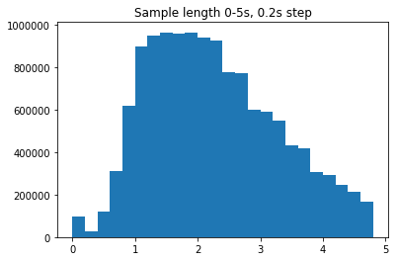
\includegraphics[width=.5\textwidth]{figures/sample0-5.png}
  \caption{Length of the samples in the dataset}
  \label{fig:samplelength}
\end{figure}

As correcting for potential errors has been crucial in the dataset preprocessing, the overlapping samples were analyzed for their characteristics.
The \cref{fig:overlapstats} shows the length of these overlaps, both in time and as a percentage of the sample.
Most of the overlapping samples had overlapped another sample completely while simultaneously being very short.
Another peak can also be seen at the beginning of the percentage graph, indicating that some samples were overlapped minimally.
Both peaks were expected to have been mostly caused by formatting and other non-dialogue content in the subtitle files.
Due to the nature of the data in the percentage graph, one overlap causes two results to appear in the graph as sample A overlaps sample B and vice versa.

\begin{figure}
    \centering
    \begin{subfigure}[b]{.45\textwidth}
        \centering
        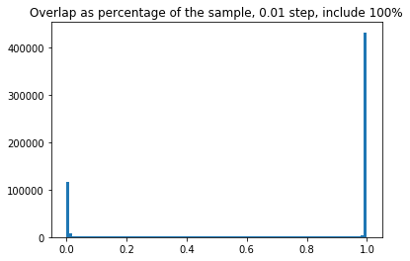
\includegraphics[width=\textwidth]{figures/overlap0-100.png}
        \caption{Percentage of the overlap in the samples}
        \label{sfig:overlappercent}
    \end{subfigure}
    \hfill
    \begin{subfigure}[b]{.45\textwidth}
        \centering
        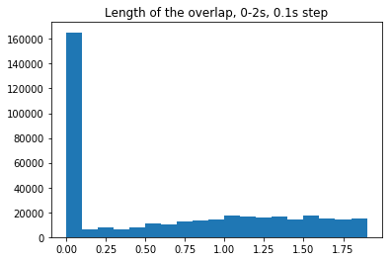
\includegraphics[width=\textwidth]{figures/length0-2.png}
        \caption{Length of the overlap in the samples}
        \label{sfig:overlaplength}
    \end{subfigure}
    \caption{Overlap statistics from the samples that had an overlap recorded}
    \label{fig:overlapstats}
\end{figure}

%Section 2: Neural network used
\section{Neural network}
During the course of this thesis, multiple neural network structures were tested with multiple parameters to determine the best network to use on the dataset.
As at the beginning of the thesis, the experience of the student with developing neural networks was negligible, which made this development process useful in both an educational and exploratory purpose.
Each of the subsections mentions the methodology used in an associated experiment.

\subsection{Early development}
%Minimal details on what happened in early dev and what was the groundwork for extra layer
%Mention marine vessels as grounds for faster development, 3 layers conv + maxpool etc
Early development of the neural network model has been a very chaotic process of learning new features of neural networks, applying them to the first experiment, and seeing what would stick.
During this time, the Classification of Marine Vessels\cite{marine} thesis written by a fellow NTNU student served as a helpful guide in using neural networks for audio processing.

%Find details on this model
The first neural network model in the thesis consisted of three dense layers, followed by the final dense output layer.
Unfortunately, this model never achieved any stable results, and rarely achieved results better than the random classification used as the control group in \autoref{ex:dataset}.
Following repeated failures, the three dense layers were replaced with one-dimensional convolution layers, all containing 64 filters and a filter size of 3.

%Also mention alexnet and googlenet, last fc layer based on that
Basing the network structure on the AlexNet\cite{Krizhevsky:2017:ICD:3098997.3065386} and Inception\cite{szegedy2014going} papers, the early model has also included a single classification layer towards the end of the model.
Since unlike Inception, the network data was not flattened during data processing throughout the network, a flattening layer was included before this classification layer.

%Mention why 10 classes were picked, 1/100 of 1000 that were used in alexnet etc, that paper that mentioned clustering, served as good start
Multiples of 1000 samples were used in the early development of the neural network model, based on the number of classes used in the papers mentioned above.
As the goal of the thesis has been to group audio samples autonomously, a dense layer representing the output layer was added to the network, with a neuron count of 10, followed by another with a neuron count of 1000.
The decision to spread the 1000 samples across ten classes was made based on the related work\cite{ClusterExample}, excluding more than 15-20 classes from being used.
The ten classes were picked to make the division into classes more simple.


\subsection{Extra layer} %Title wip
\label{me:exlayer}
%APW report territory, experiment 2 results
%Theoretical walkthrough ONLY, experiment chapter details work done and why
As the early model was only designed to handle 1000 samples, and it did not carry any capacity to grow to learn more, a modification was done to the final output layer of the network.
Instead of 1000 neurons, the network was expanded to carry 1010 neurons, with the final ten being manually modified to transfer the results from the softmax layer directly to the final output layer.

An illustration of this can be seen in \cref{fig:extralayerexample}.

\begin{figure}[htbp]  % order of priority: h here, t top, b bottom, p page
  \centering
  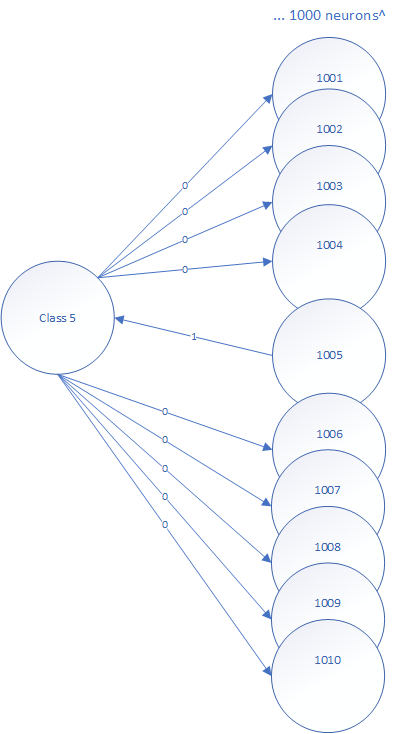
\includegraphics[width=.5\textwidth]{figures/Drawing1.png}
  \caption{Example of the 1010 neuron layer}
  \label{fig:extralayerexample}
\end{figure}

%Explain theory
By manually modifying the weights to translate the results of the network to the last layer, parts of the dataset that have been classified already can be used by assigning them to the last ten classes.
The manual weights in the layer prevent any significant modification from being done by the training optimizer to the classifications of these last neurons while leaving the first 1000 free to be changed.
The only values that the optimizer can use to classify the new dataset are the values provided by the softmax layer, meaning that the samples have to be assigned by the optimizer to be one of these ten classes.
As the new dataset is trained on with the old dataset, the weights cannot be adjusted to the point of overfitting by the new dataset.
However, some adjustment is desired, as these adjustments can be picked up on by the iterative re-training process to improve the neural network as a whole.

An experiment detailed in \cref{ex:layer} was conducted to verify this layer in practice

\subsection{Final model}
%Spring model dev, explain the more thorough work on the model, setting up multiple layers, how many layers
%Experiment 3 detailing results and how the work went, no mention of this here
%Goal is good validation accuracy and low validation loss, should acc or loss be similar the goal is to aim for both
%Mention that it was at this stage that agg clustering was brought in to stabilize the results
Following the development of the extra layer, the final neural network model for this thesis was developed.
Since the earlier model was built very quickly to make decisions about parts that were needed to develop the final model, with those parts in place, the final model could be put together.

Operational variables were identified in the various components used in a convolutional neural network to develop the neural network model that would be suited for the task it would work on, 
As running all of the possible variable combinations would take forever, determining the correct number of convolutional layers was deemed the top priority.
The full details on the process of selecting the optimal network configuration are listed in \cref{ex:networkref}.

\subsubsection{Stabilizing the result}

In the beginning, it was intended that the neural network would do its classification from the very first iteration, generating the initial clusters by itself.
While it was determined that the network is capable of doing this in \cref{ex:dataset} and \cref{ex:layer}, the results were not stable and predictable.
Each run on the same data would return a different cluster, meaning that comparing two different configurations of neural networks would be mostly meaningless.
The first cluster has been from this point onward generated using the Scikit-learn Agglomerative clustering function to bring stability to the network, and to make the results more predictable.



%Two "main" sections, first section from autumn semester, second from spring semester
%First section define the early "model" built with the help of marine paper
%First section refers to experiment 2, which details on the results for the custom layer
%Second section refers to experiment 2 producing good results, final layer being used
%Selection of the network model done by repeatedly attempting multiple combinations of parameters
%Display a list of parameters tested

%Detail the methodology used in creating the "base" neural network used in this thesis

%Section 3: Loss function
\section{Loss function}
The loss function modifications have been a central part of the development part of the thesis.
As the custom layer has proven in \cref{ex:layer} that a custom part can significantly improve the performance of the training process, the same has been assumed for the loss function modifications.

%Filter
\subsection{Primary filter}
The filter in the loss function targets the results of the network after a top-K function has sorted them.
To prevent the filter from damaging the result of the current class, that class is excluded from the filter.
As the results are sorted highest to lowest, the filter adds an extra penalty to the result by multiplying the result with itself.
In the case of the highest values, the penalty is inverted, as the cost of errors is significantly reduced.
The goal of the filter was to incentivize the network to cluster samples more equally by penalizing massive clusters and rewarding the smaller ones.

%Pictures of the filters
\cref{fig:me:loss01} and \cref{fig:me:loss23} show the filters used in the thesis, following the results of \cref{ex:loss}.
Filter 0 (\cref{sfig:me:loss0}) is a simple forgiveness filter that removes the penalty of the first 200 samples.
Filter 1 (\cref{sfig:me:loss1}) is a similar filter, except the final 200 samples are penalized doubly.
Filter 2 (\cref{sfig:me:loss2}) is the first gradual increase filter, where the filter gradually progresses towards a defined point at a constant rate, and then changes the rate once somewhere in the middle of the filter.
Filter 3 (\cref{sfig:me:loss3}) is based on a similar concept as filter 2; however, it also has a shelf similar to filter 1 in the middle of it.

The first two filters are meant to investigate the steep increase in penalties and rewards, while the last two filters are meant to investigate the gradual increase in penalties and rewards.

\begin{figure}
    \centering
    \begin{subfigure}[b]{.45\textwidth}
        \centering
        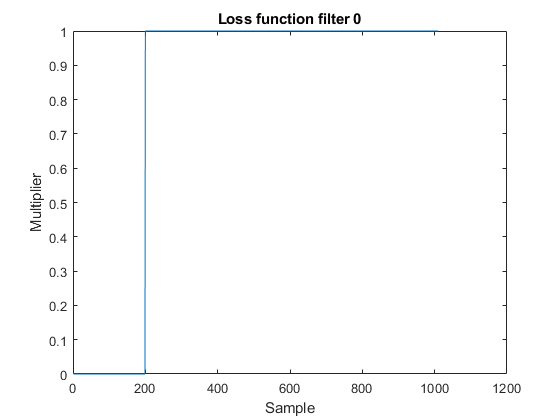
\includegraphics[width=\textwidth]{figures/loss-0.png}
        \caption{Loss function filter 0}
        \label{sfig:me:loss0}
    \end{subfigure}
    \hfill
    \begin{subfigure}[b]{.45\textwidth}
        \centering
        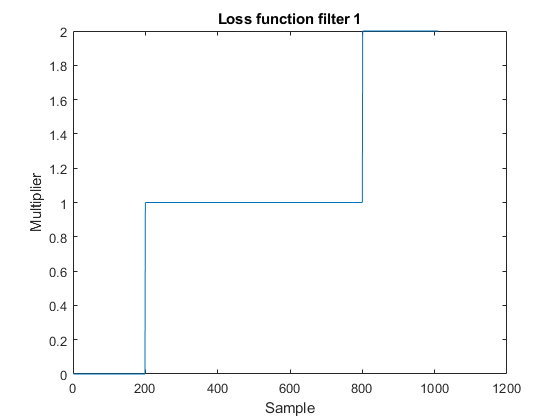
\includegraphics[width=\textwidth]{figures/loss-1.png}
        \caption{Loss function filter 1}
        \label{sfig:me:loss1}
    \end{subfigure}
    \caption{Loss function filters 0 and 1}
    \label{fig:me:loss01}
\end{figure}

\begin{figure}
    \centering
    \begin{subfigure}[b]{.45\textwidth}
        \centering
        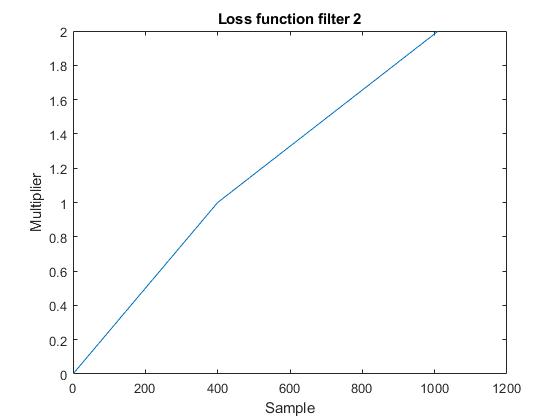
\includegraphics[width=\textwidth]{figures/loss-2.png}
        \caption{Loss function filter 2}
        \label{sfig:me:loss2}
    \end{subfigure}
    \hfill
    \begin{subfigure}[b]{.45\textwidth}
        \centering
        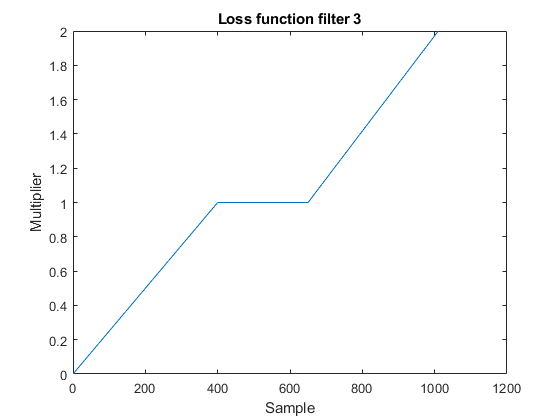
\includegraphics[width=\textwidth]{figures/loss-3.png}
        \caption{Loss function filter 3}
        \label{sfig:me:loss3}
    \end{subfigure}
    \caption{Loss function filters 2 and 3}
    \label{fig:me:loss23}
\end{figure}


%Second filter
\subsection{Second filter}
\label{me:secondfilter}
In addition to the primary filter, another filter has been added to the loss function.
As the last ten neurons are not the normal sample neurons, these need to be treated differently.
The most substantial value among these ten neurons has its loss function cost removed, to guide the network to group samples according to these groups.
A sub-experiment in \cref{ex:loss:secondfilter} has aimed to add an extra cost to the remaining nine neurons that would follow after the first.
However, the experiment has yielded inconclusive towards negative results as to the usefulness of this second filter increase.
Thus, the second filter only removes the first of the ten final neurons from the loss function cost.


%In detail provide information on how I created my custom loss function filters, tuned the parameters
%Here is NOT the reason I went down from 10 classes to 3
%Explain the logic behind the filter types, show graphs that can illustrate some of this
%Generate graph with gnuplot like in example, more natural?
%Explain the logic behind the filter values, why these in particular
%Include second filter explanation, subexperiment of loss function experiments


%Q: Provide this info 10->3 in methods or results? IMO methods but can see how it would be relevant in results

\section{Iterative re-training}
\label{me:iter-retrain}
%Section 4: Iterative training
%Explain the purpose, massive dataset that can't fit in memory, would take forever to train
Iterative re-training has been considered critical to the thesis due to the sheer size of the dataset.
While the dataset could be reduced to fit more efficiently during the training process, it would ultimately be a tiny percentage of what was available.
A good part of the value in the research done in this thesis is the large dataset involved, and therefore it was critical to at least attempt this.

%For the purpose of grouping data, it would be mostly superfluous, after the initial batch of data most samples should have a definitive cluster
Given the objective of the thesis, iterative re-training was considered to be the right choice regardless of the dataset size.
While one can always achieve a better cluster distribution if one throws more data at the algorithm, odds are the cluster generated with only a couple thousand samples will be relatively close, at a fraction of the computational cost.
Additionally, the data that does not fit well into any of the existing clusters is likely to have the most significant effect on the network, meaning that these are the samples that carry the most substantial significance.


%The samples that don't fit the threshold are added to the small train dataset
The goal of the iterative re-training process was to start with a minimal dataset and work through the dataset, accumulating new knowledge as more data is parsed.
As more data is processed, more samples appear out of the norm and are absorbed into the training dataset.
Over time, the new samples would give insight into better clustering adjustments that would prevent some of the samples that were yet to be processed, to be inserted into the dataset.


%The hypothesis is that the change in samples that were already certain is not huge, and possibly becomes more certain with more retraining, while samples that were uncertain become more certain even further down the dataset
%subsection for parameters used, reference results from previous experiment for loss functions, plus threshold, control versions -1 and -2

%First of the two sort of relevant to the results sections
%Specify the parameters used in determining the correct parameters in developing iterative training
A parameter has to be picked that will determine if a sample is important enough to be considered for use in the dataset, or if it should be ignored to start the process of iterative re-training,
In the thesis report, this parameter is referred to as the "Iteration threshold."
If the iteration threshold is set to 0.8, for example, any sample that is classified higher than the threshold will be ignored for use in the dataset, while samples classing lower will be added to the dataset.

%Specify what loss functions and parameters would used in iterative training depending on what results

Following the decision on the iteration threshold parameter, the process of iterative re-training follows these steps:
\begin{enumerate}
    \item Train the first network using a pre-determined method
    \item Classify samples until the minimum amount of valid samples are detected
    \item Re-classify the samples using the selected process
    \begin{enumerate}
        \item Samples can also not be re-classified. Instead one can use the results of the first classification
    \end{enumerate}
    \item Train the network using the bigger dataset
    \item Return to step 2 until the entire dataset is processed
\end{enumerate}

The experiment detailing the practical parts of the iterative re-training can be found in \cref{ex:iter-retrain}.

\section{Tree generation}
%Section 5: Tree generation
%Tree generation, same as iterative training in terms of specifying what I did, results of this goes into results/discussion
%Specify what iterative training parameters will be used depending on the criteria in the results
%The hypothesis is that over time, samples that get grouped together will be more and more similar, either by pure values or at least with sample text ("Hello") samples get grouped together into a cluster somewhere
%Subsection for tested parameters, mention final experiment detailing this
%Based on iterative train, mention what would be used to prune some of the combinations for trees, angle towards 0.8


